\chapter{Materials and Methods}

In this section we describe the steps required to get from a primary protein sequence to its tertiary structure.
It begins with the description of the input and the motivation for using it. 
Second part focuses on the model choices and mainly describes the convolutional neural network. 
The last section focuses on the structure realization. 
A graphical overview of the entire pipeline is showed in Figure \ref{fig:project_pipeline}. 
In each of the 3 subsections the corresponding part of the diagram will be unraveled to accompany the verbal descriptions.

\begin{figure}[ht]
    \centering
    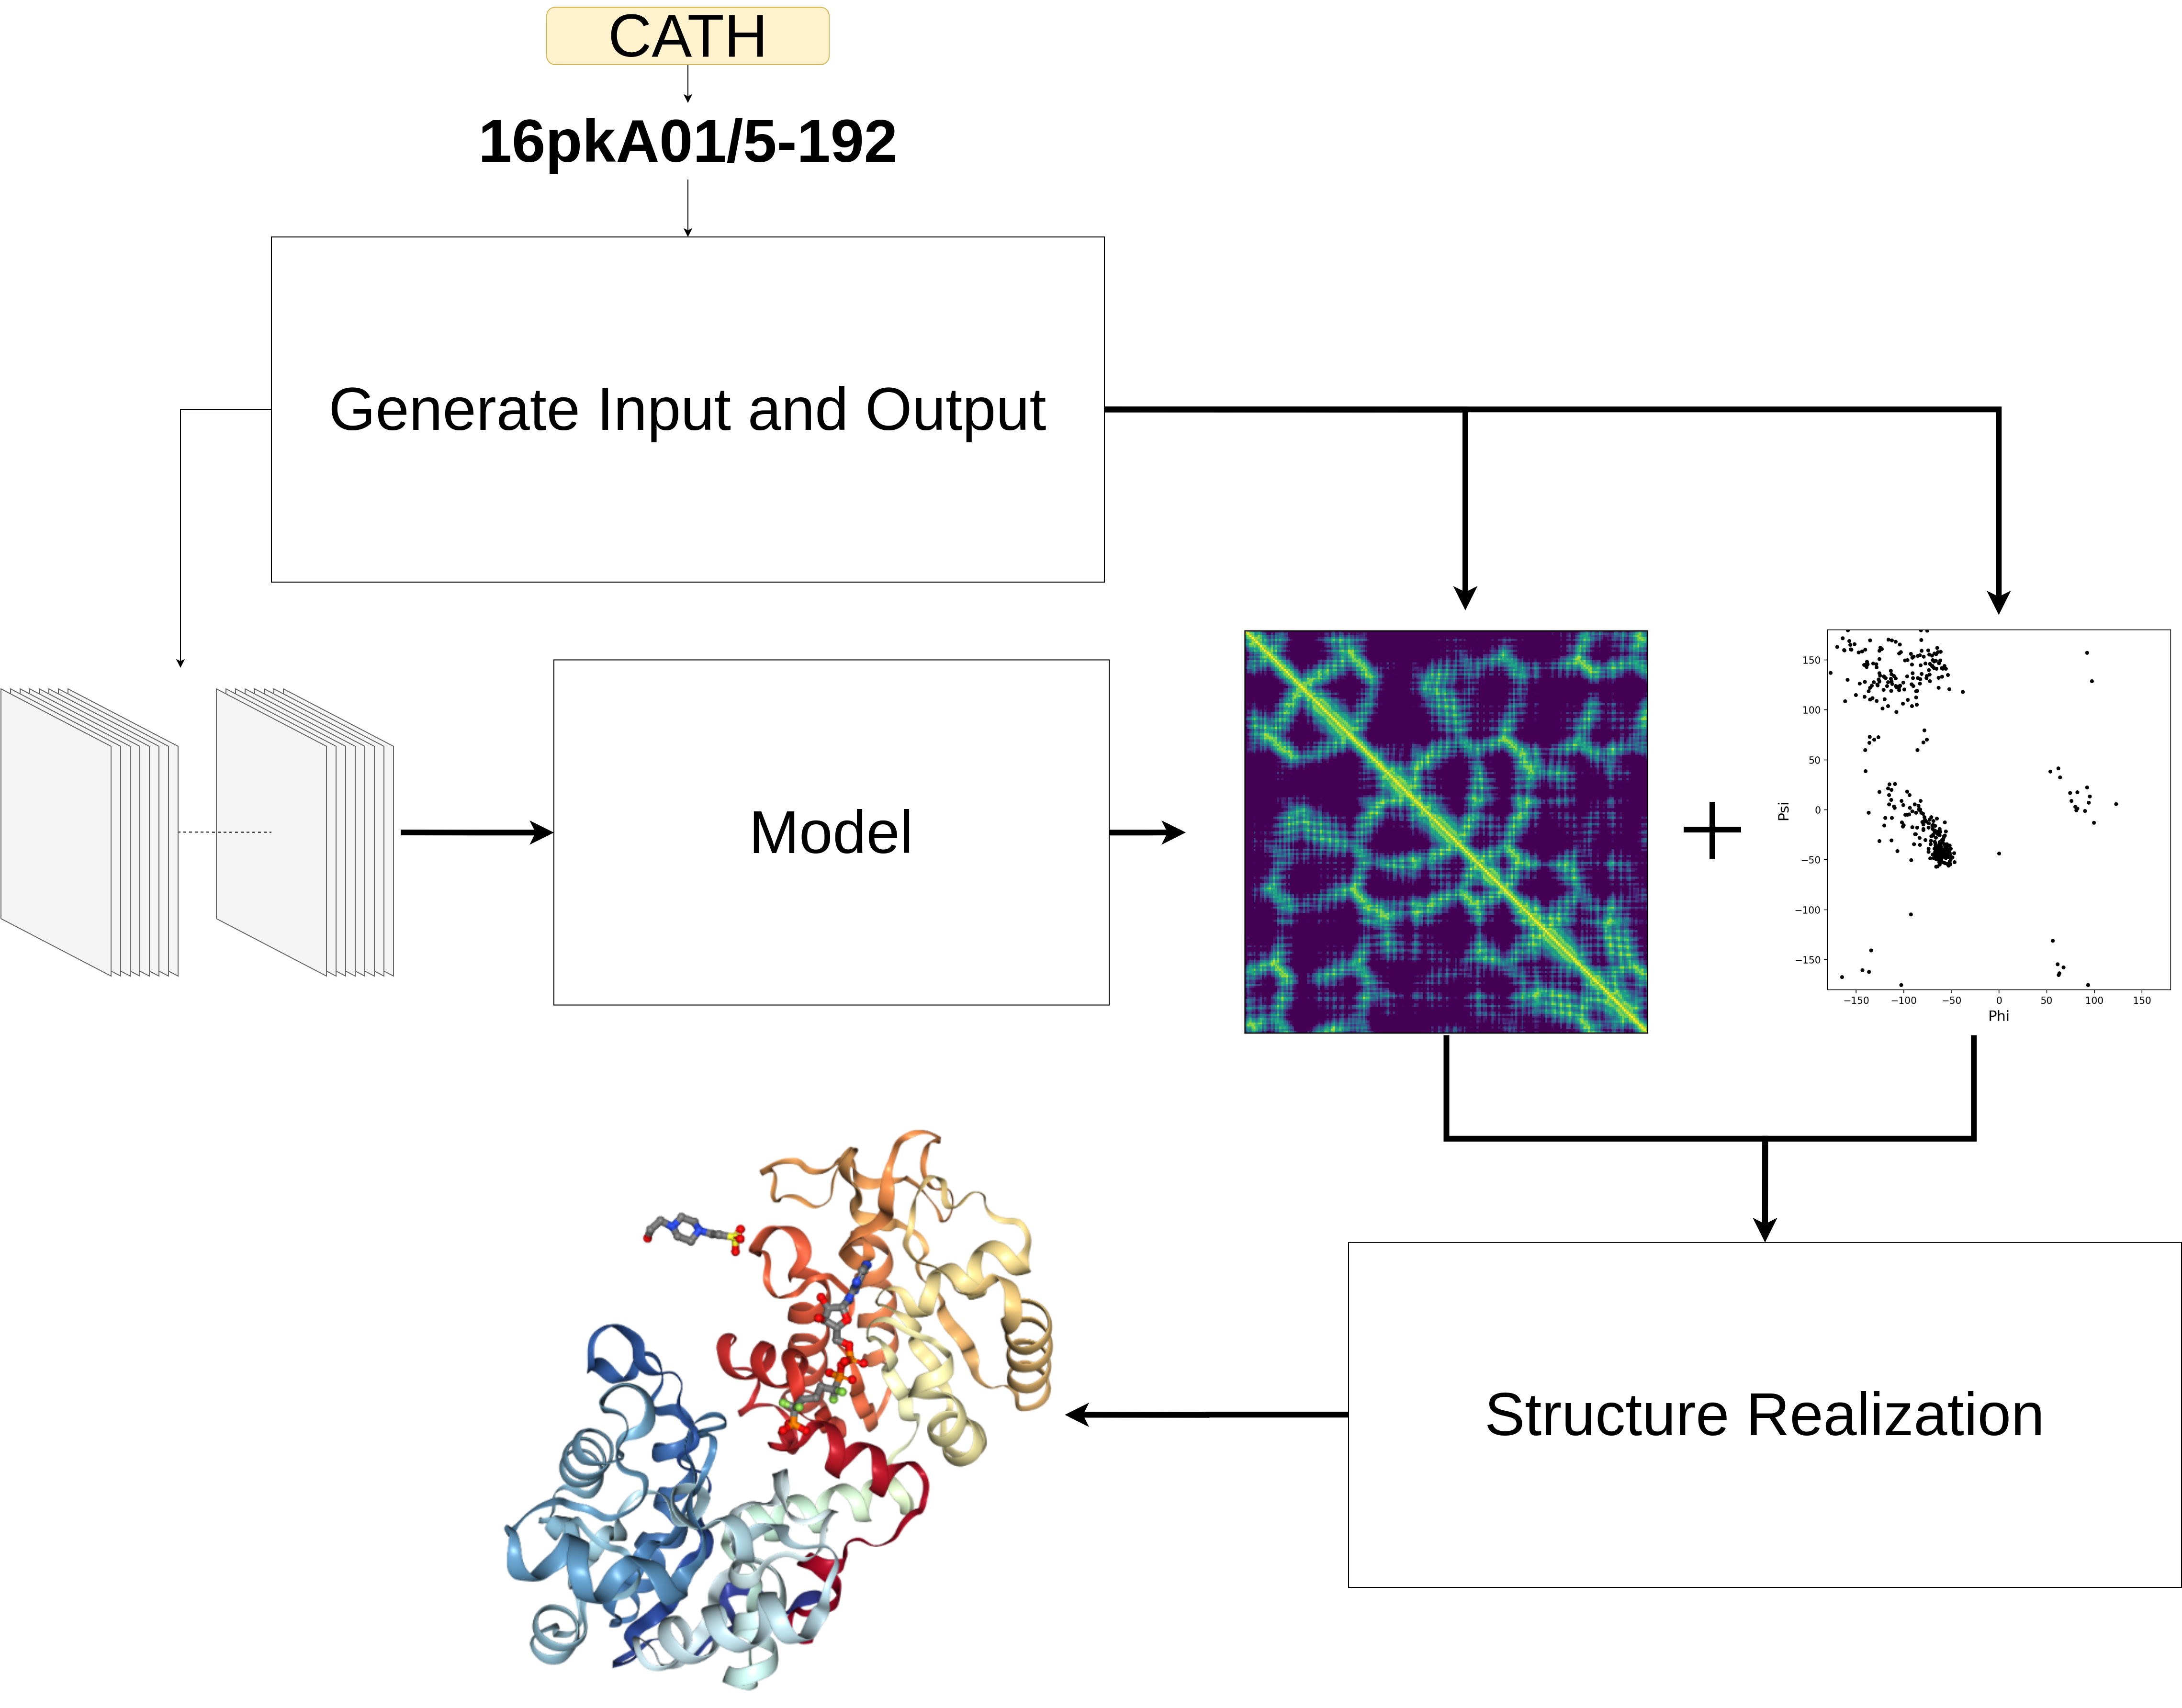
\includegraphics[width=0.8\linewidth]{imgs_tomas/Project_pipeline_small.png}
    \caption{Pipeline overview}
    \label{fig:project_pipeline}
\end{figure}

\section{Primary Sequence to CNN Input}

During evolution, we expect that functional parts of proteins are going to be conserved. 
Furthermore, we expect that two amino acids that are close to each other in the 3D space (not necessarily in the primary sequence) are going to co-evolve as well. 
This co-evolution of spatially proximal amino acids should be reflected in the Multiple Sequence Alignment (MSA) of a protein. 
In order to generate a MSA for a selected domain, one has to first find proteins that share some ancestry with it (homologs), which is done by searching through database of sequences and picking proteins that have certain sequence similarity. 
From these sequences we can generate the MSA.
    
From the MSA we can calculate the propensities of amino acids at each position of the sequence very easily, which yields the Postion Specific Scoring Matrix (PSSM). 
To model the interaction we can use the Direct Coupling Analysis (Potts model).
    
This section is going to be organised as follows. 
We are first going to explain how to search for similar proteins and construct the MSA using the HHblits tool. 
The second part will focus on the MSA summary statistics such as PSSMs and Potts Models. 
In the last part we will discuss the encoding of the input, so that it is ready for use in the convolutional neural network.
    
\subsection{Available data}
% \section{Data used for training and model evaluation}
    
\begin{figure}[b!]
    \centering
    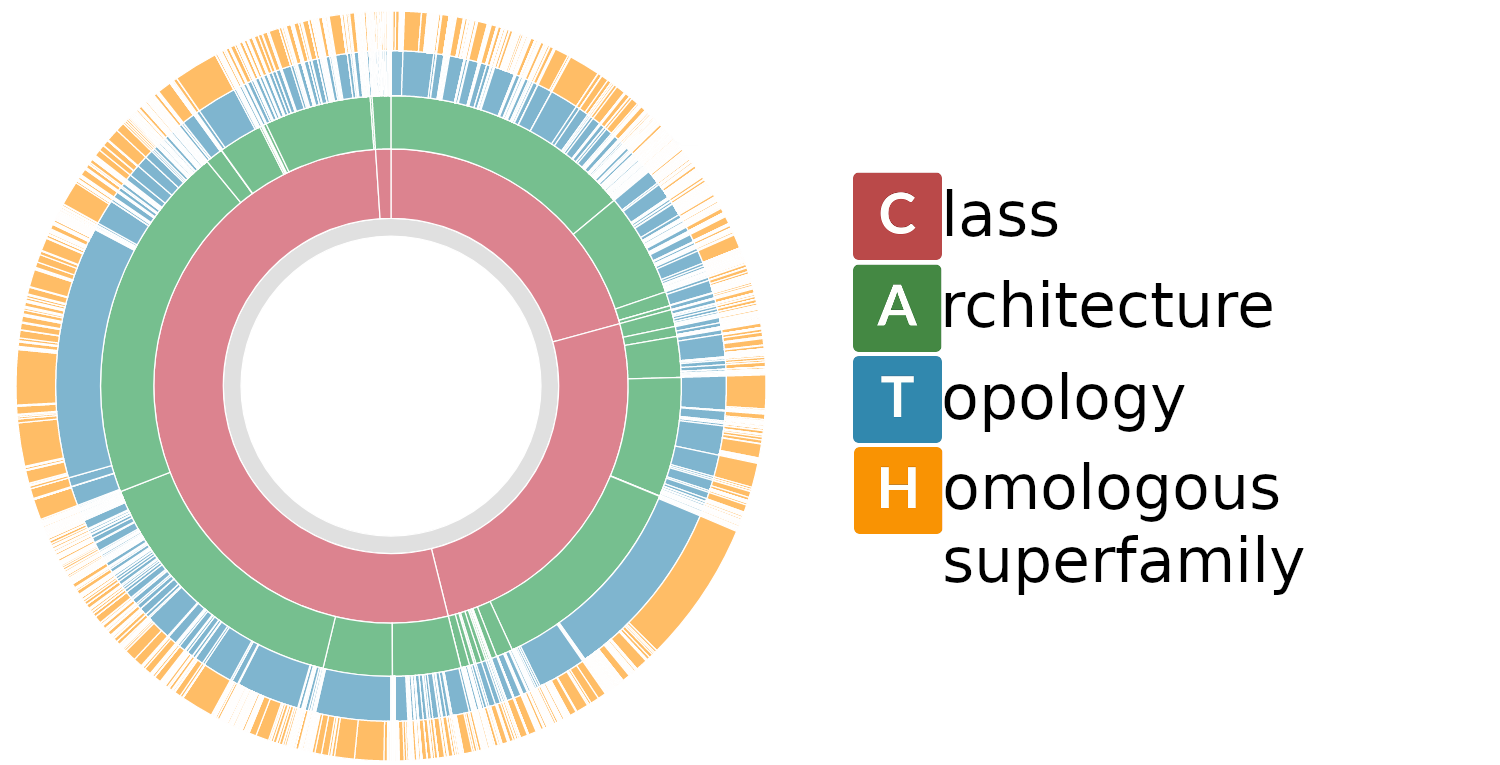
\includegraphics[width=\linewidth]{imgs_tomas/cath.png}
    \caption{CATH hierarchy \cite{cath}}
    \label{fig:cath}
\end{figure}
    
For training we used protein sequences from the CATH S35 dataset. 
CATH is a database that clusters proteins with known structures based on 4 criteria: Class (secondary structure classes), Architecture (secondary structure arrangement in 3D space), Topology (how secondary structure elements are connected) and Homologous Superfamily (evolutionary relationship between domains). 
Figure \ref{fig:cath} shows the hierarchical relationship between the classes.
    
To ensure dataset diversity, we used a dataset of sequences with pairwise sequence similarity of at most 35\% (hence the S35). 
The list of domains together with their sequences in \texttt{fasta} format can be accessed at: \href{ftp://orengoftp.biochem.ucl.ac.uk/cath/releases/latest-release/sequence-data/cath-domain-seqs-S35.fa}{oregonftp.biochem.ucl.ac.uk}.
    
Domains are short regions of proteins that fold more or less independently of each other. 
The \texttt{fasta} file contains for each domain its protein name, chain identifier and the domain ranges. 
This information is crucial for downloading and preparing the structures from Protein Data Bank database. 
Two example headers are shown below. 
    
\begin{center}
    \texttt{>cath|4\_2\_0|1a41A02/217-310}\\
    \texttt{>cath|4\_2\_0|3lnnA01/12-42\_283-342}
\end{center}
    
These two examples show domains - \texttt{1A41} and \texttt{3LNN}, downloaded from the CATH database version 4.2.0. 
The next letter (\texttt{A} in both cases) represents the chain and the last two characters are the domain id, since a chain can consist of several domains. 
The full dataset (version from Sept. 4 2017) consists of 31289 domains. 
    
We decided to exclude segmentated domains from the dataset and also the ones with missing PDB coordinates. 
This resulted in a set of 19953 domains. 
Looking at the sizes of homologous superfamilies in Figure \ref{fig:cath}, there are few large ones (like the immunoglobulin family in bottom left with more than 8000 domains) and the rest are relatively small (less than 50). 
Our model works woth evolutionary data (MSA - PSSMs/Potts), which means that having a overrepresented family in the data set might introduce some biases that might make the model generalization more difficult. 
For this reason we decided to impose an exclusion threshold (= 500), where in families with more members we randomly picked "exclusion threshold" of domains out of them. 
After this filtering, the dataset size reduced to 11014 domains. 
The distributions of CATH classes can be seen in Figure \ref{fig:cath_filtered}.
    
\begin{figure}
    \centering
    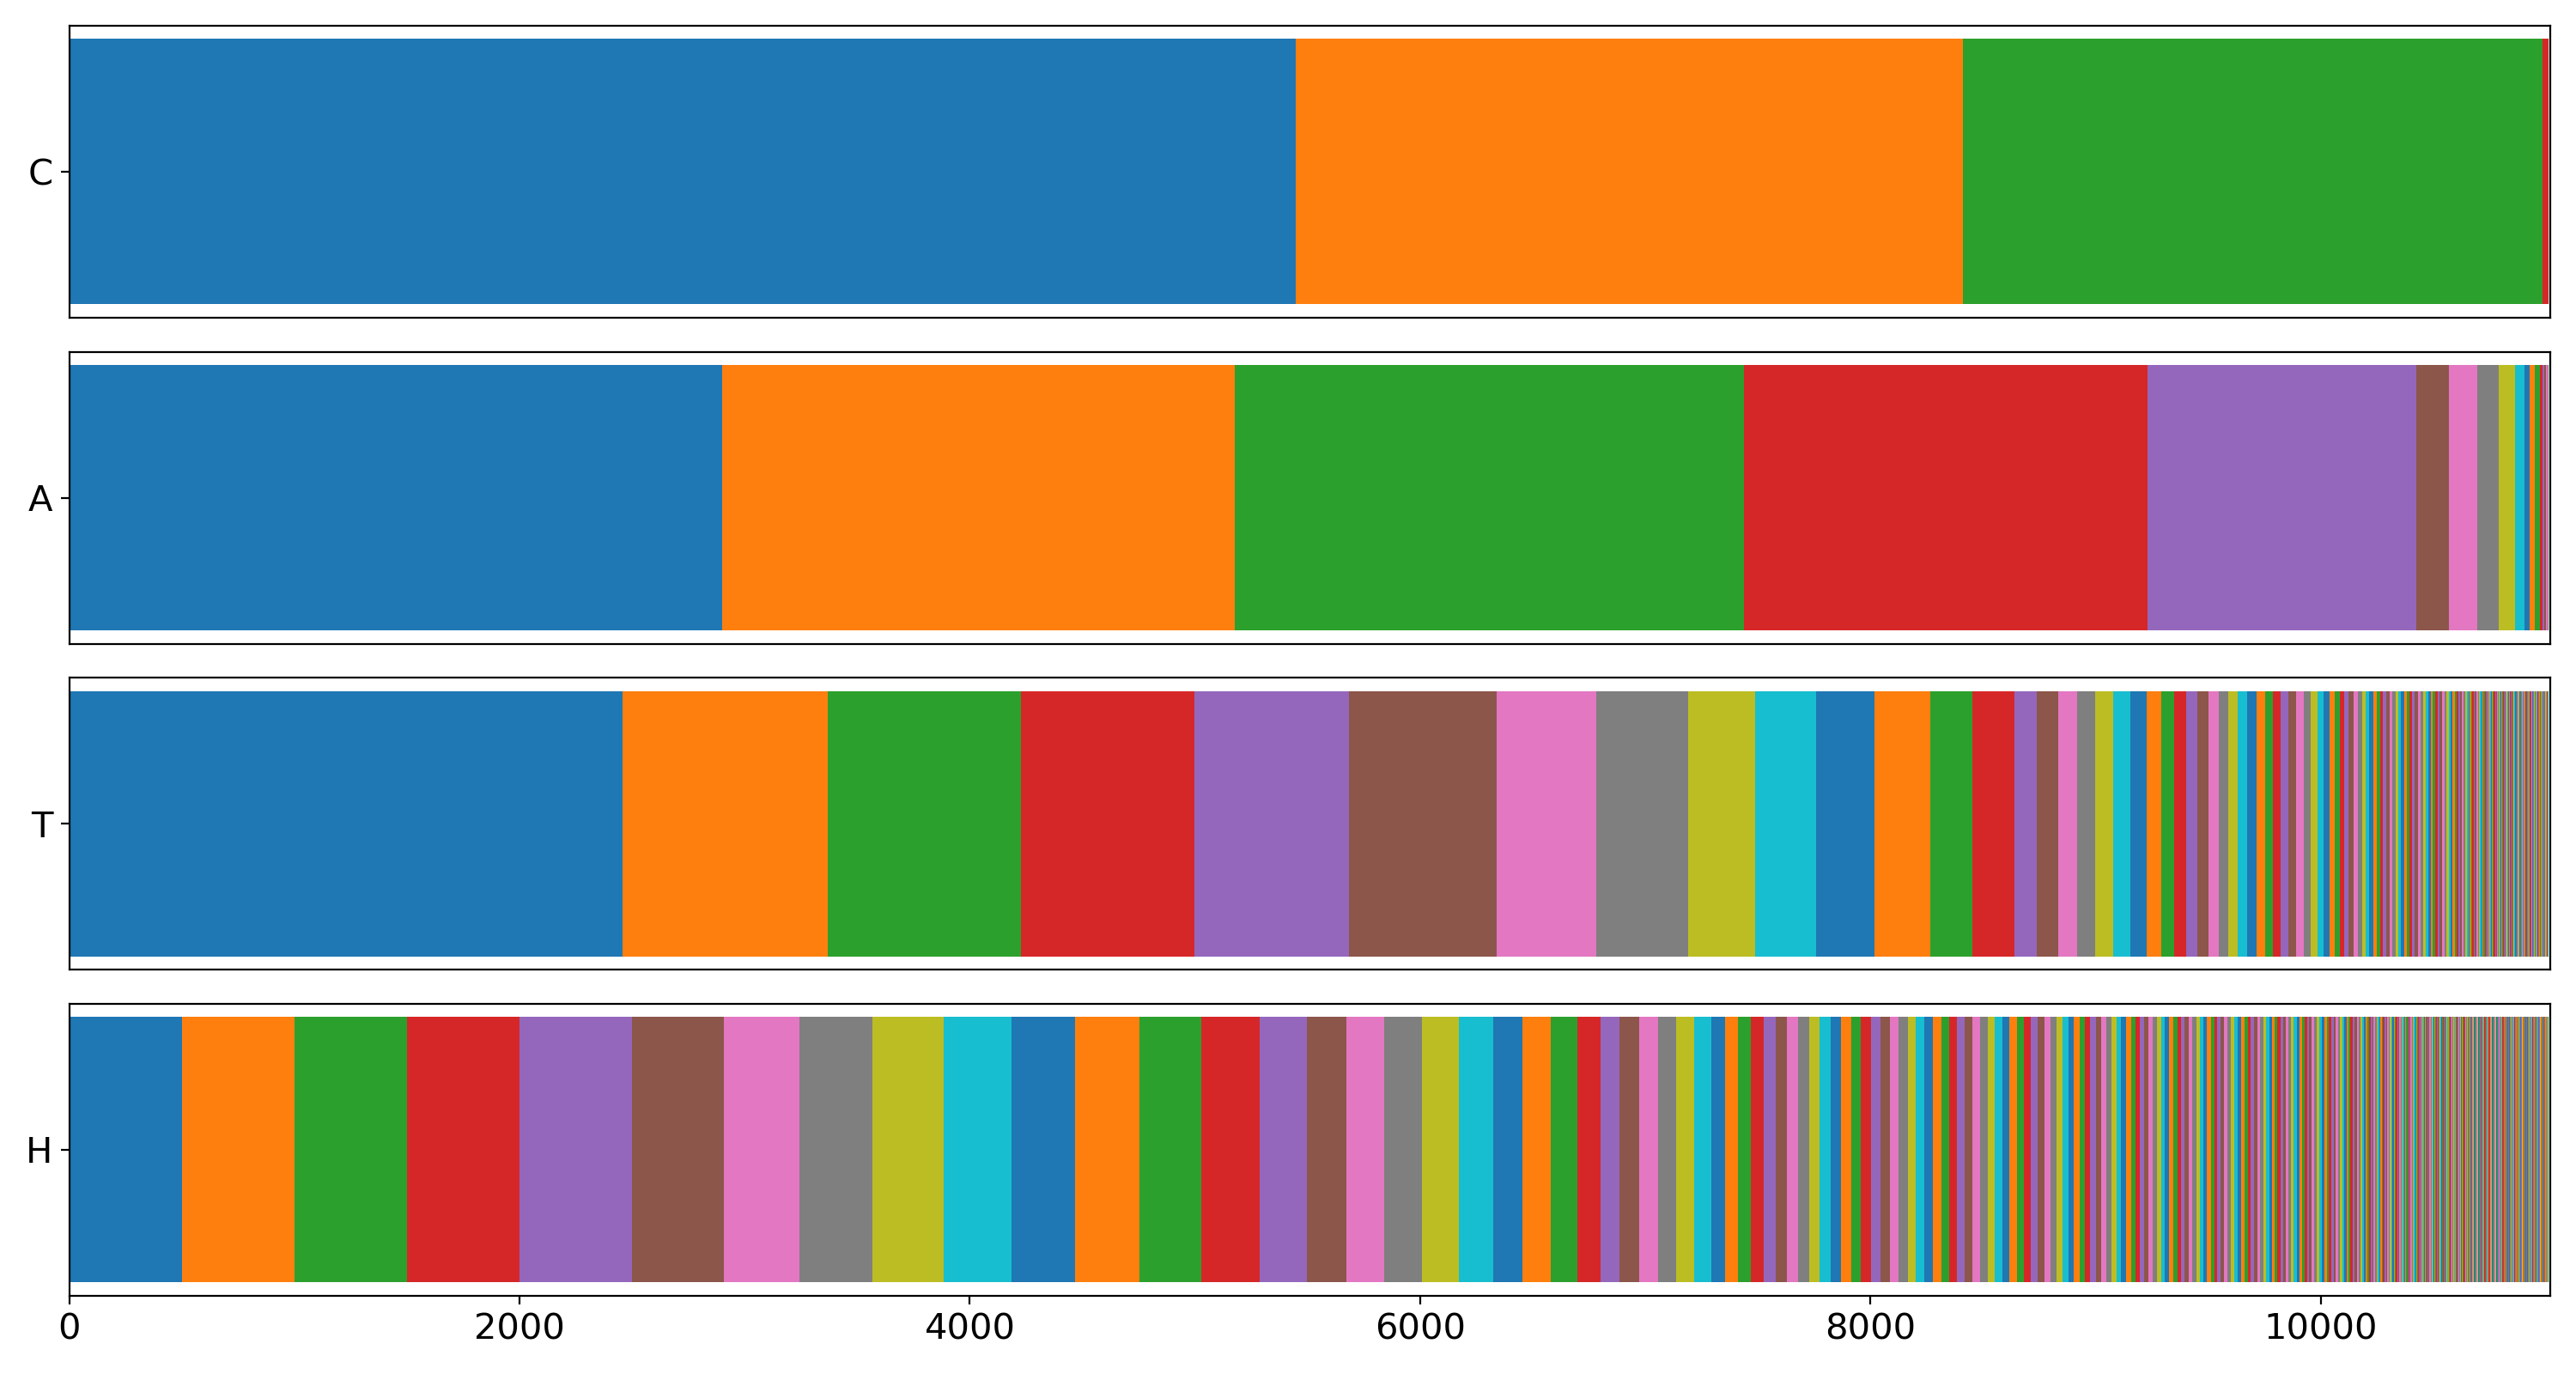
\includegraphics[scale=0.4]{imgs_tomas/cath_distributions_filtered.png}
    \caption{Caption}
    \label{fig:cath_filtered}
\end{figure}

\subsection{Sequence search and MSA}


\subsection{Potts Models}

Lets assume that we have a sequence $\boldsymbol{\sigma} = (\sigma_1, \sigma_2, ..., \sigma_L)$, where $L$ is the length of the multiple sequence alignment. 
Lets further assume that each symbol $\sigma_i$ in the sequence comes from an alphabet $\mathcal{A} = (a_1, a_2, ..., a_Q)$ of size $Q$. 
Thus for sequence length $L$ we can generate $Q^L$ number of unique sequences.
    
In our case, the sequence $\boldsymbol{\sigma}$ is some sequence of amino acids, and thus the alphabet size is equal $Q = 21$ (20 amino acids, 1 gap symbol).
        
Given a MSA, we would like to find pairs of amino acids that are coupled, ie. the pairs of amino acids that are correlated due to their direct contact. 
The reason why we can not use correlation data directly, is that some pairs of amino acids might be correlated through some intermediate paths.
        
We have to keep in mind that MSA is only generated from a sample of sequences. 
Thus it can only help us to estimate the frequencies and connected correlations of amino acids. 
To calculate the connected correlation of a pair of amino acid, we can use the covariance formula:
            
$$c_{ij}(k, l) = f_{ij}(k, l) - f_i(k) f_j(l)$$
        
where
$$f_i(k) = \frac{1}{B} \sum_{i = 1}^B \delta(\sigma_i^{(b)} = k)$$
$$f_{ij}(k, l) = \frac{1}{B} \sum_{i = 1}^B \delta(\sigma_i^{(b)}, k)\delta(\sigma_j^{(b)}, l)$$
        
calculate the frequency of symbol $(k)$ and pair of symbols $(k, l)$ at position $(i)$ and positions $(i, j)$ in the MSA. 
$\delta(\sigma_i^{(b)}, k)$ is an indicator function that is equal to one when $\sigma_i^{(b)} = k$.
        
% add example
        
Our goal is to create a model: $\mathcal{P(\bm{\sigma})}$ that can reproduce the observed frequencies. 
The constraints of the model are:
        
$$\mathcal{P}(\sigma_i = k) = \sum_{\substack{\bm{\sigma}\\ \sigma_i = k}} \mathcal{P}(\bm{\sigma}) = f_i(k)$$
$$\mathcal{P}(\sigma_i = k, \sigma_j = l) = \sum_{\substack{\bm{\sigma}\\ \sigma_i = k \\ \sigma_j = l}} \mathcal{P}(\bm{\sigma}) = f_{ij}(k, l)$$
        
The model that satisfies these constraints and has the maximal information entropy is called a Potts Model:
        
\begin{equation}
    \mathcal{P}(\bm{\sigma}) = \frac{1}{\mathcal{Z}} exp\left(\sum_{i = 1}^{L-1} \sum_{j=i+1}^L \bm{J}_{ij}(\sigma_i, \sigma_j) + \sum_{i=1}^L \bm{h}_i({\sigma_i})\right)
    \label{eq:Potts}
\end{equation}
    
In this equation, $\mathcal{Z}$ is the normalizing constant/partition function that ensures that the probabilities sum to 1. 
The parameters of the model $\bm{J}$ and $\bm{h}$ describe the pairwise interactions and propensities respectively.
        
To find the parameters of a model that best describe the observed MSA, we can define a loss function:
        
\begin{equation}
    \mathcal{L} = -\frac{1}{B} \sum_{i=1}^B logP(\bm{\sigma}^{(b)})
    \label{eq:potts_loss}
\end{equation}
        
Specifically for Potts Model: 
        
\begin{equation}
    \mathcal{L}_(\bm{h}, \bm{J}) = log \mathcal{Z} - \sum_{i = 1}^L \sum_{k \in \mathcal{A}} f_i(k)\bm{h}_i(k) - \sum_{i = 1}^{L-1} \sum_{j=i+1}^L \sum_{k, l \in \mathcal{A}} f_{ij}(k, l) \bm{J}_{ij}(k, l)
    \label{potts_loss_ml}
\end{equation}
        
This loss function is differentiable and so we seek to find its minimum. 
However, to do so, we need to know the value of the partition function ($\mathcal{Z}$), which is practically incomputable for larger domains. 
Therefore its approximation is required.
        
Instead of considering the entire space of possible sequences, we can ask about the probability of a certain symbol in a sequence in MSA ($\sigma_r^{(b)}$) knowing the rest of symbols in the sequence ($\bm{\sigma}_{\setminus r}^{(b)}$). 
The probability function in (\ref{eq:potts_loss}) becomes:
        
$$
P(\sigma_{r} = \sigma_r^{(b)} | \bm{\sigma}_{\setminus r} = \bm{\sigma}_{\setminus r}^{(b)}) = \frac{exp \left(h_r \sigma_r^{(b)} + \sum_{\substack{i = 1\\i\neq r}}^L J_{ri}(\sigma_r^{(b)}, \sigma_i^{(b)})\right)}{\sum_{q \in \mathcal{A}} exp \left(h_r(q) + \sum_{\substack{i = 1\\i\neq r}}^L J_{ri}(q, \sigma_i^{(b)})\right)}$$
        
This function is again, differentiable, although it does not minimize the loss defined in (\ref{eq:potts_loss}).
However, as opposed to \ref{potts_loss_ml}, this objective function can be computed in reasonable time with gradient descent techniques (either first order optimization or second order optimization approximation via algorithms such LBFG-S)\cite{potts1, potts2}.
        
\subsection{Position-specific Scoring Matrix}

Position-specific Scoring Matrix (PSSM) is generally used to represent biologically important patterns across multiple sequences. 

To create the PSSM, let us assume that we already constructed a multiple sequence alignment (MSA) of our target sequence and related proteins.
This multiple sequence alignment consists of $N$ rows representing sequences and $L$ columns representing positions of alignment.
Furthermore, each sequence is a sequence of letters from an alphabet with $Q$ symbols.

Then, the first step in creation of PSSM is the calculation of the Position Frequency Matrix (PFM), by simply counting the number of occurences of a symbol at a position in the MSA.
Formally, PFM is a matrix with $Q$ rows and $L$ columns, where each entry $\PFM_{q, l}$ is given by Equation \ref{eq:pfm}.

\begin{equation}
    \PFM_{q, l} = \sum_{n = 1}^{N} \delta(\MSA_{n, l}, q)
    \label{eq:pfm}
\end{equation}

From the PFM, a Position Probability Matrix (PPM) is then created simply by scaling the counts by the number of sequences in the MSA.
Therefore:

\begin{equation}
    \PPM_{q, l} = \frac{1}{N} \PFM_{q, l}
\end{equation}

The PSSM is then defined as the log likelihoods of the PPM transformed by some background model $b$.
For example, the simplest background model might be the one, where each symbol appears in the sequences equally likely, thus $b_q = \frac{1}{Q}$.
This definition gives us the Equation \ref{eq:pssm}.

\begin{equation}
    \PSSM_{q, l} = \log_2 \frac{\PPM_{q, l}}{b_q}
    \label{eq:pssm}
\end{equation}

In practice, more complex background models, such as the total frequency of a symbol in the entire MSA, is often used.
Moreover, it is often encountered, especially when number of sequences in the MSA is small, that some entries of the PFM are zeroes.
This is an issue, because it renders some sequences impossible even though they might be just very unlikely and due to the limited number of samples not observed.
To address this issue, pseudocounts are often used.
This means that we start the PFM construction with one assigned to every entry instead of zero.
It will ensure that the probabilities in the PPM will be non-zero and it also accounts for finite sample size.


% Position Probability Matrix $\mathcal{F} = \{f_{ij}\}$ with $L$ rows (target sequence length) and $Q$ columns (alphabet size). 
% Each entry in the matrix is a frequency of occurence of a symbol in the current position in the MSA:
        
% $$f_i^*(k) = \frac{1}{B} \sum_{b = 1}^B \delta(\sigma_i^{(b)}, k)$$

% In both cases,  the  influence  of  pseudocounts  declines  with  the  size  of  the  training  set  (√N/N  in  the  first  case,  0.1/N  in  the  other),  which  is  just  what  you  would  want,  since  the  purpose  of  pseudocounts  is  to  diminish  the  distortions  inherent  in  using  a  small  training  set.  The  higher  the  value  of  B,  the  more  sequences  will  be  found  (including  perhaps  some  real  binding  sites  that  might  otherwise  be  missed)  but  at  the  cost  of  diluting  the  impact  of  what  is  known  about  the  binding  site.  Lower  values of B thus produce fewer false positives.
        
% To ensure that there are no zero probabilities in the final matrix, pseudocounts are added. 
% If $u_k$ is the occurence of a symbol in the entire MSA and $C$ is some arbitrary constant (usually equal to $\sqrt{L}$ or $0.1$), the frequency can be calculated as:
% $$f_i(k) = \frac{B(f_i^*(k) + u_k C)}{B + C}$$
        
% The items in PSSM are then defined as:
        
% $$PSSM_i(k) = log_2\left(\frac{f_i(k)}{u_k}\right)$$
        
% (\href{http://www.people.vcu.edu/~elhaij/IntroBioinf/Notes/PSSM.pdf}{http://www.people.vcu.edu/~elhaij/IntroBioinf/Notes/PSSM.pdf})
        
% (\href{https://en.wikipedia.org/wiki/Position_weight_matrix#cite_note-Stormo1982-1}{WIKI})
        
% \section{Data used for training and model evaluation}
    
% \begin{figure}[b!]
%     \centering
%     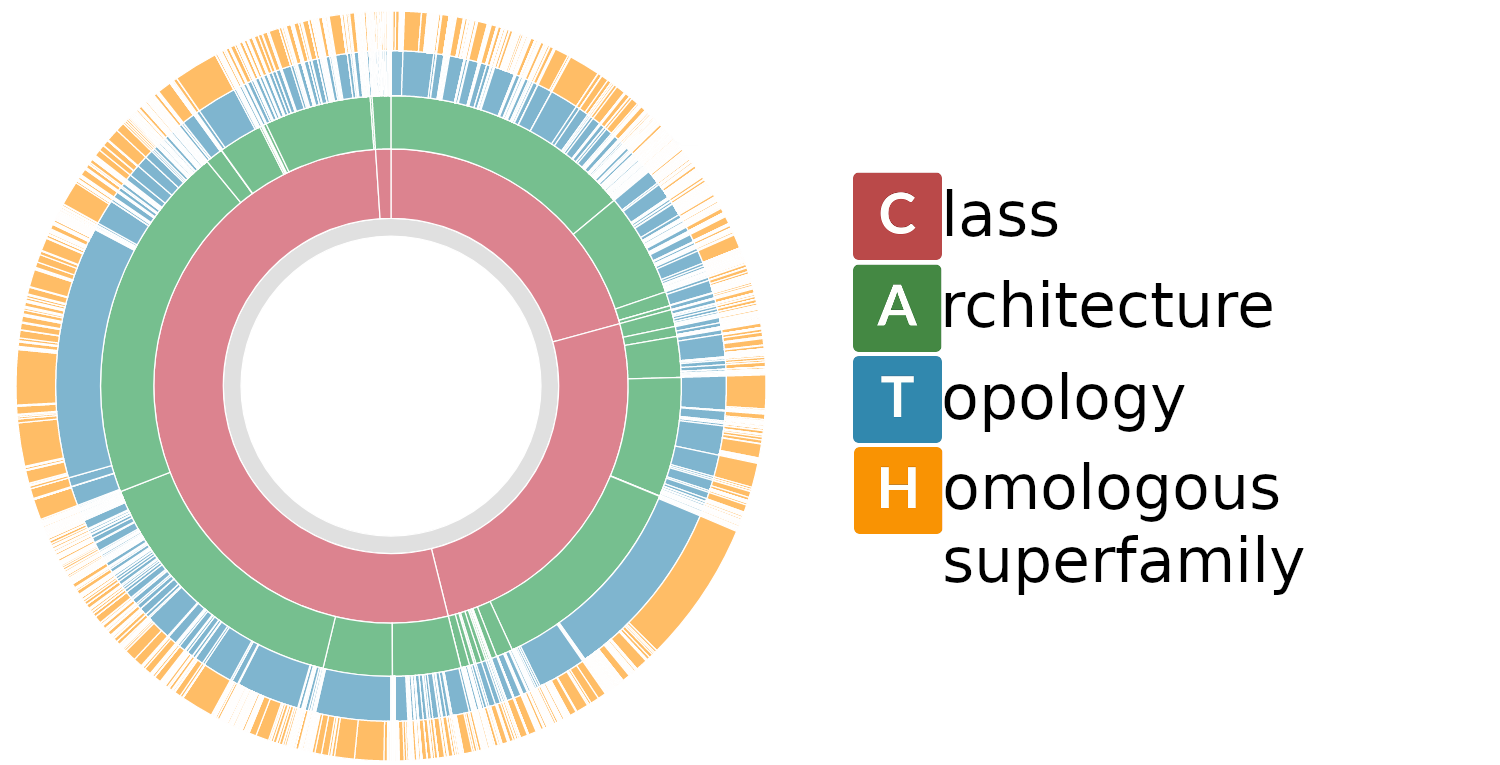
\includegraphics[width=\linewidth]{imgs_tomas/cath.png}
%     \caption{CATH hierarchy \cite{cath}}
%     \label{fig:cath}
% \end{figure}
    
% For training we used protein sequences from the CATH S35 dataset. 
% CATH is a database that clusters proteins with known structures based on 4 criteria: Class (secondary structure classes), Architecture (secondary structure arrangement in 3D space), Topology (how secondary structure elements are connected) and Homologous Superfamily (evolutionary relationship between domains). 
% Figure \ref{fig:cath} shows the hierarchical relationship between the classes.
    
% To ensure dataset diversity, we used a dataset of sequences with pairwise sequence similarity of at most 35\% (hence the S35). 
% The list of domains together with their sequences in \texttt{fasta} format can be accessed at: \href{ftp://orengoftp.biochem.ucl.ac.uk/cath/releases/latest-release/sequence-data/cath-domain-seqs-S35.fa}{oregonftp.biochem.ucl.ac.uk}.
    
% Domains are short regions of proteins that fold more or less independently of each other. 
% The \texttt{fasta} file contains for each domain its protein name, chain identifier and the domain ranges. 
% This information is crucial for downloading and preparing the structures from Protein Data Bank database. 
% Two example headers are shown below. 
    
% \begin{center}
%     \texttt{>cath|4\_2\_0|1a41A02/217-310}\\
%     \texttt{>cath|4\_2\_0|3lnnA01/12-42\_283-342}
% \end{center}
    
% These two examples show domains - \texttt{1A41} and \texttt{3LNN}, downloaded from the CATH database version 4.2.0. 
% The next letter (\texttt{A} in both cases) represents the chain and the last two characters are the domain id, since a chain can consist of several domains. 
% The full dataset (version from Sept. 4 2017) consists of 31289 domains. 
    
% We decided to exclude segmentated domains from the dataset and also the ones with missing PDB coordinates. 
% This resulted in a set of 19953 domains. 
% Looking at the sizes of homologous superfamilies in Figure \ref{fig:cath}, there are few large ones (like the immunoglobulin family in bottom left with more than 8000 domains) and the rest are relatively small (less than 50). 
% Our model works woth evolutionary data (MSA - PSSMs/Potts), which means that having a overrepresented family in the data set might introduce some biases that might make the model generalization more difficult. 
% For this reason we decided to impose an exclusion threshold (= 500), where in families with more members we randomly picked "exclusion threshold" of domains out of them. 
% After this filtering, the dataset size reduced to 11014 domains. 
% The distributions of CATH classes can be seen in Figure \ref{fig:cath_filtered}.
    
% \begin{figure}
%     \centering
%     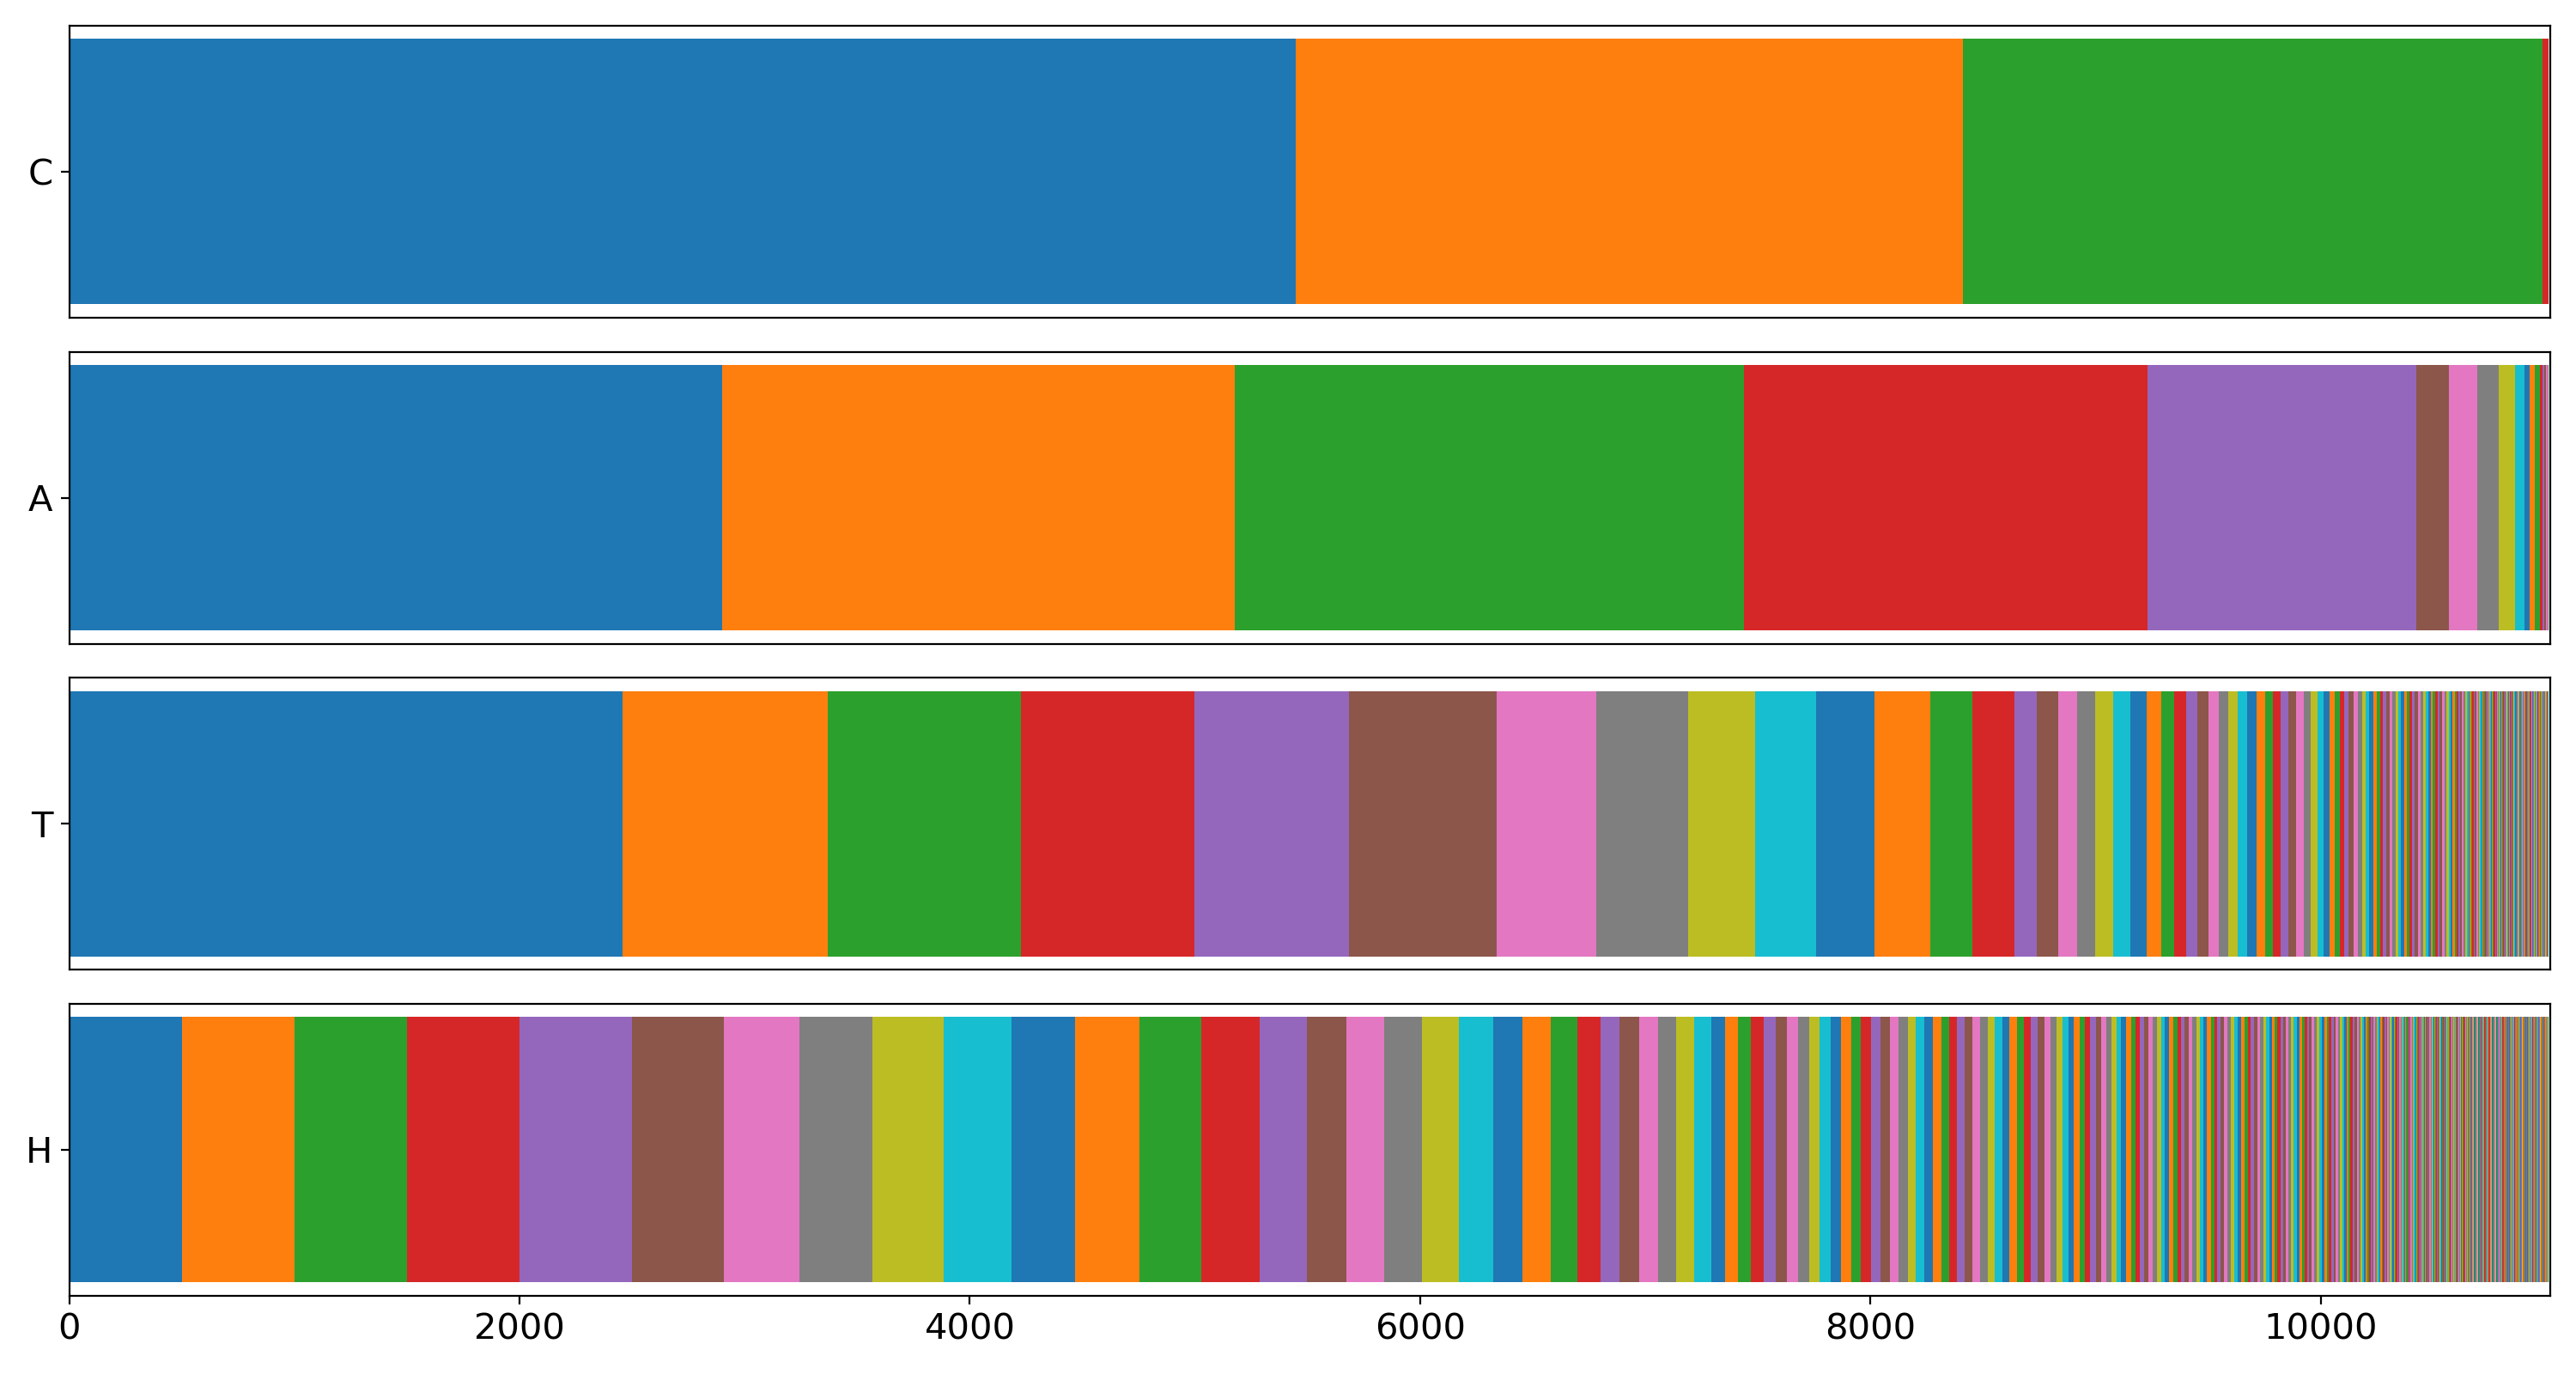
\includegraphics[scale=0.4]{imgs_tomas/cath_distributions_filtered.png}
%     \caption{Caption}
%     \label{fig:cath_filtered}
% \end{figure}
    
\subsection{Train/Validation/Test split}
    
In the AlphaFold paper \cite{alphafold}, the authors decided to create train/validation/test set of homologous superfamilies instead of randomly picking the domain. 
The rationale behind this is to include all members of each homologous superfamily in either training, validation or test set. 
This ensures that when evaluating the model performance of a set of proteins, that very similar proteins were not used for training. 
    
We decided to train our models on a set of 9514 domains. 
We tried several models and neural network architectures. 
After picking the most promising ones, we evaluated their performance on a validation set of 1000 domains. 
We picked the best model and trained on both training and validation data and finally estimated the model performance on a test set of 500 domains. 
We take this as a final decising metric and error of the model. 
    
Furthermore, to simulate the famous CASP (Critical Assessment of protein Structure Prediction) competition we downloaded the domains used in in CASP13 from 2018. 
We can be sure that these domains were not used in training because the CATH domain list we downloaded was uploaded in September 2017. 
We picked 24 domains from the Regular Targets category.
    
\subsection{Input encoding}
To give a short summary, our input consists of:
    
\begin{itemize}
    \item One-hot-encode sequence of shape $(L, 21)$
    \item Positions $(i, j)$ of shape $(2, L, L)$
    \item PSSM of shape $(L, 20)$
    \item Potts $\bm{J}$ of shape $(L, L, 21, 21)$
    \item Potts $\bm{h}$ of shape $(L, 21)$
    \item Potts Frobenius Norm of $\bm{J}$ of shape $(L, L)$
\end{itemize}
        
Since we want to take into consideration effects of spatially distant amino acid pairs, we would like to generate an input tensor of shape: $(Channels, L, L)$.
    
\subsection{Output encoding}
        
\subsubsection{Distance maps}
The labels used for training were downloaded from the Protein Data Bank (PDB) which offers rich description of many proteins, including their tertiary structure. 
Most of the structures were determined via X-Ray crystallization technique which is not always able to fully describe the structure. 
Thus many proteins have many missing atomic coordinates. 
        
For the reasons of structure realization and residue placement, AlphaFold (and also ProSPr) extracted the C$_\beta$ coordinates of the residues (C$_\alpha$ for glycine) \cite{alphafold}.
        
Although distance is a continuous measure, and it would make perfect sense to treat the problem as a regression one, AlphaFold discretized the distances into 64 bins ranging from 2 to 22\AA, with one bin used for distances larger than 22\AA and one bin for missing data. 
The reason for doing so becomes clearer after understanding how the structure realization (the last step of the entire pipeline) was performed.
    
\begin{itemize}
    \item PDB database
    \item Discretization of distances
\end{itemize}
        
\subsubsection{Secondary structure and torsion angles}
        
The secondary structure was classified into 8 categories suggested by DSSP (Dictionary of Protein Secondary Structure). 
The categories are shown in table \ref{tab:dssp}.
        
\begin{table}[ht]
    \centering
    \begin{tabular}{c|c}
        DSSP code & Secondary Structure\\ 
        \hline
        H     & $\alpha$-helix \\
        B     & Isolated $\beta$-bridge residue \\
        E     & strand \\
        G     & 3-10 helix \\
        I     & $\Gamma$-helix \\
        T     & Turn \\
        S     & Bend \\
        -     & Other 
    \end{tabular}
    \caption{DSSP Secondary Structure Classes}
    \label{tab:dssp}
\end{table}
        
On top of the secondary structure classification, the output of the DSSP program also conveniently includes the torsion angles $\phi$ and $\psi$.
        
\section{Structure Realization}
    
This is the final step of the entire pipeline. 
Knowing that the tertiary structure can be fully described by its torsion angles, we would like to find a set of torsion angles so that the induced inter-residue distances are as close as possible to the predicted ones. 
        
This explanation should clarify the decision of treating the inter-residue distance prediction (and torsion angles) as a classification problem rather than as a regression one. 
Instead of predicting a single number, we decided to generate a histogram of distances and torsions. 
In the next step the authors of the AlphaFold paper fitted a 3rd-degree spline the distograms and von-Misses distribution \footnote{von Mises distribution is a continouous distribution defined on a circle in range $[0, 2\pi)$ with a bell like shape. Formally its probability density function is $\mathds{P} = \frac{e^{\kappa cos(x - \mu)}}{2\pi I_0(\kappa)}$ where $I_0(\kappa) = \sum_{i=0}^\infty \frac{\kappa^{2i}}{2^{2i}(i!)^2}$ is a modified Bessel Function with order zero. 
The $\kappa$ parameter is a called concentration and describes the dispersion. 
$\mu$ is the mean direction of the distribution \cite{vonmises}} to the torsion angles distributions. 
This is a neccessary step that ensures the smoothness of the distributions and allows the calculation of partial derivatives.
        
We would like to create a model of the protein structure - $\mathcal{G}(\phi, \psi)$ ($\phi$ and $\psi$ are the torsion angles) which returns the distances between residues. 
These induced distance should be as close as possible to the predicted ones (together with the torsions). 
Thus we can define a loss function/potential:
        
\begin{equation}
    V(\phi, \psi) = V_{dist}(\mathcal{G}(\phi, \psi)) + V_{torsion}(\phi, \psi)
\end{equation}
        
where \cite{alphafold}(supplementary information):
        
\begin{equation}
     V_{dist}(\mathcal{G}(\phi, \psi)) = -log\left(\sum_{i, j, i \neq j} \mathds{P} (d_{ij} | S, MSA(S)\right)
\end{equation}

\begin{equation}
    V_{torsion}(\phi, \psi) = -log\left(\sum_{i, j, i \neq j} \mathds{P}_{von Mises} (\phi, \psi | S, MSA(S)\right)
\end{equation}
        
Since this is an optimization problem, we can approach a good solution with a gradient descent algorithm. 
Because there are so many possible protein conformations, the optimization is highly influenced by the initial conditions. 
The torsion angles can be sampled from the predicted distributions and ideally the optimization process is run several times.  
        
\subsection{Simplified case in 2D}
Lets imagine the protein as a string of beads, where the beads right next to each other are constant distance away - lets call it $r$. 
Any conformation of such string can be fully described by the signed successive polar angles - see Figure \ref{fig:struct_real2d}.
        
\begin{figure}[ht]
    \centering
    \includegraphics[scale=0.22]{imgs_tomas/simplified_2d.png}
    \caption{Caption}
    \label{fig:struct_real2d}
\end{figure}
        
The left part of the figure introduces the notation when working with complex numbers. 
The right part shows an arrangement of 5 residues in 2D space. 
The grey-filled circles represent amino acid residues and the black vectors are the connections between residues of constant size $r$. 
The first vector (connecting residue 0 and residue 1) is anchored at the origin. 
The colorized vectors coming from the origin are translated versions of the remaining vectors. 
        
In order to compute the distance between two residue, for example distance between residiue 0 and residue 4 (shown as a dotted line on the right hand side of the Figure \ref{fig:struct_real2d}) we need to add the contributions of every vector between those two points, ie:
        
$$\bm{d_{0,4}} = \bm{d_{0,1}} + \bm{d_{1,2}} + \bm{d_{2,3}} + \bm{d_{3,4}}$$
        
The magnitude of a complex number can be easily calculated from the Pythagorean formula:
        
\begin{equation}
    |z|^2 = x^2 + y^2 = cos^2(\theta) + sin^2(\theta)
    \label{eq:complex_magnitude}
\end{equation}
        
The distance (in general) is:
        
\begin{equation}
    d_{i,j}^2 = r^2 |\bm{d_{0,1}} + \bm{d_{1,2}} + ... + \bm{d_{j-2,j-1}} + \bm{d_{j-1,j}}|^2
    \label{eq:dist_gen}
\end{equation}
        
In complex representation (using both equation \ref{eq:complex_magnitude} and \ref{eq:dist_gen}):
        
\begin{equation}
    d_{i,j}^2 = r^2 \left|\sum_{k=i}^j cos(\theta_k) + i sin(\theta_k)\right|^2 = r^2 \left[\left(\sum_{k=i}^j cos(\theta_k)\right)^2 + \left(\sum_{k=i}^j sin(\theta_k)\right)^2\right]
    \label{eq:dist_2d}
\end{equation}
        
\subsection{Simplified case: 3D}
        
In 3D, the case is almost the same as in 2D, we just need use another angle ($\phi$) to fully describe the arrangement. 
The transformation of Cartesian coordinates to polar is:
        
$$x = r cos(\theta) sin(\phi)$$
$$y = r sin(\theta) sin(\phi)$$
$$z = r cos(\phi)$$
   
The distance between two residues $i$ and $j$ in 3D is (just as in the 2D case) the magnitude of a vector pointing from residue $i$ to residue $j$. 
This vector is again the sum of all vectors between these two residues. 
Similarly to equation \ref{eq:dist_2d}, the formula for calculating (squared) distance between two residues in 3D is:
        
\begin{equation}
    d_{i,j}^2 = r^2 \left[\left(\sum_{k=i}^j cos(\theta_k) sin(\phi_k)\right)^2 + \left(\sum_{k=i}^j sin(\theta_k) sin(\phi_k)\right)^2 + \left(\sum_{k=i}^j cos(\phi_k)\right)^2\right]
\end{equation}
        
\subsection{Full Model}

\section{Train/Validation/Test split}
    
\section{Neural Networks}

\begin{itemize}
    \item Why Neural Networks?
\end{itemize}

\subsection{Basic FCNN}

\begin{itemize}
    \item Forward, Loss, Backward, parameter initialization
    \item Activations
    \item weights/parameters
\end{itemize}

\subsection{CNN}

\begin{itemize}
    \item Channels, Conv layers, Pool layers
\end{itemize}

\subsection{ResNets}
    
\subsection{AlphaFold}
    
\section{Structure Realization}
\subsection{Naive approach}
pca - eigenvalue decomposition - tomas will explain
\subsection{Contact maps for struct realization}
state of the art 3 years ago
there is an app for pc
\subsection{LBFGS}
\subsection{Potentials}
